
\documentclass[journal]{IEEEtran}
\usepackage{blindtext}
\usepackage{graphicx}
\usepackage[utf8]{inputenc}
\usepackage[italian]{babel}

\ifCLASSINFOpdf
\else
\fi

\hyphenation{op-tical net-works semi-conduc-tor}


\begin{document}
\title{Creazione ed analisi di una metodologia per la progettazione di interfacce utente per Sistemi Embedded di fascia bassa}

\author{Enrico Giordano,~\IEEEmembership{Università degli Studi di Verona}}
%\thanks{Davide Quaglia} 
%\thanks{Graziano Pravadelli}% <-this % stops a space


\maketitle


\begin{abstract}

La progettazione di interfacce utente per Sistemi Embedded ha avuto un notevole sviluppo per renderle sempre più gradevoli ed efficienti, avvicinandosi sempre più ai concetti di portabilità e mantenibilità tipica dei sistemi General Purpoise. Si tende sempre più ad investire su processori di fascia media per poter utilizzare tecnologie tipicamente Client-Server, in modo da poter trattare le applicazioni basate su grafica in maniera più modulare possibile in accordo con le ultime tecnologie, soprattutto usando la rete e protocolli di rete standard, come HTTP. Questo però risulta problematico in tanti sistemi di fascia bassa, in cui l'ottimizzazione è essenziale per la corretta progettazione, ma anche per i vincoli non funzionali da rispettare, rendendo scorrette le tecnologie attualmente utilizzate. Si vuole quindi proporre un metodo per la progettazione di questi sistemi, con un framework appositamente creato per analizzare le performance e la velocità di progettazione.

\end{abstract}
\IEEEpeerreviewmaketitle



\section{Introduzione}

Esistono due categorie di Sistemi Embedded in commercio:
\begin{itemize}
\item dispositivi ciechi, che non sono dotati di schermo e non permettono quindi di presentare un'interfaccia;
\item dispositivi visuali, che sono dotati di schermo e permettono di presentare un'interfaccia.
\end{itemize}

Nonostante ciò, esistono varie tecniche per presentare un'interfaccia utente per comandare il dispositivo o semplicemente presentare lo stato della macchina. Il metodo più antico e tipico dei Sistemi Embedded consiste nel creare un terminale testuale comandato via comandi seriali a caratteri; un esempio può essere il terminale comandato via UART. Con la definizione di protocolli di rete, si è sentita la necessità di utilizzarli per garantire robustezza e sicurezza, oltre ad avere la possibilità di avere un'interfaccia multiutente e facilmente portabile ed implementabile. Ultimamente quindi utilizzare un'interfaccia di rete con protocollo standard come HTTP è uno standard \textit{de facto}.

Il problema però sorge quando si hanno risorse talmente limitate da non permettere l'utilizzo di alcune tecnologie tipicamente moderne, come la programmazione ad oggetti o stack di rete completi; quindi nasce la necessità di avere delle implementazioni più ottimizzate e semplici, sia per dispositivi ciechi, sia per dispositivi visuali.

\subsection{Sistemi Embedded di fascia bassa}

Dal momento che un'azienda sceglie di utilizzare un tipo di Sistema Embedded di fascia bassa per motivi ragionevoli, cioè i costi di produzione, il progettista embedded deve tenere conto di vari vincoli, tra cui:

\begin{itemize}
\item vincoli realtime, ovvero il sistema deve rispondere entro un certo limite di tempo;
\item vincoli di memoria, ovvero non eccedere con il codice compilato dal punto di vista di spazio occupato;
\item vincoli di consumo, ovvero non si deve consumare troppa energia per eseguire un'operazione.
\end{itemize}

Rispettare questi vincoli è molto difficile, quindi solitamente si spende molto tempo e quindi risorse per progettare una \textit{business logic} che implementa la logica del sistema, ma è ancora più tedioso progettare un'interfaccia grafica per comandarla e controllarla.

%Come caso di studio di questo progetto, è stato scelto un processore di fascia bassa della NXP, ovvero LPC1788, che permette di essere sia dispositivo cieco, sia dispositivo visuale, grazie la sua GPU integrata per gestire un dispositivo come uno schermo LCD Touch.

\subsection{Librerie utilizzate}

Poichè i Sistemi Embedded da commercializzare necessitano di progettazione abbastanza veloce, in accordo con le regole del \textit{time to market}, varie aziende mettono a disposizione diverse librerie commerciali ottimizzate per gestire al meglio le interfacce o, più in generale, la progettazione stessa del sistema. In generale, per progettare un Sistema Embedded, è necessario conoscere nella sua interezza il microprocessore, però vengono fornite delle API per astrarre il più possibile il device. 

Per la progettazione di interfacce per sistemi di fascia bassa, commercialmente si utilizza una libreria grafica chiamata EmWin, offerta dalla SEGGER. Questa si basa sul paradigma di programmazione ad eventi, in modo da evitare di utilizzare necessariamente un sistema operativo. La progettazione può avvenire in due modalità diverse:

\begin{itemize}
\item hard coded, ovvero scrittura completamente manuale sia della grafica sia della business logic associata;
\item soft coded, ovvero disegnando l'interfaccia il "GuiBuilder", programma in dotazione, per poi scrivere manualmente le funzioni associate all'interazione con i widget.  
\end{itemize}

Per la progettazione della parte di rete, esiste una libreria leggera e ottimizzata che implementa il protocollo TCP/IP, ovvero LWIP. Questo si propone come standard per i disposivi di fascia bassa che necessitano di rete ma non hanno abbastanza risorse disponibili per ospitare l'intero stack di rete TCP/IP. 

Per la progettazione rapida di Sistemi Embedded, esiste un framework chiamato uEZ (si pronuncia come ``Muse'' in Inglese) che offre un'astrazione dell'hardware per progettare ad alto livello il sistema. Questo racchiude le librerie precedenti in modo da offrire un ambiente completo per lo sviluppo, mascherando tutte le possibili chiamate a basso livello tramite API. Questo lo si può rappresentare con il seguente schema:

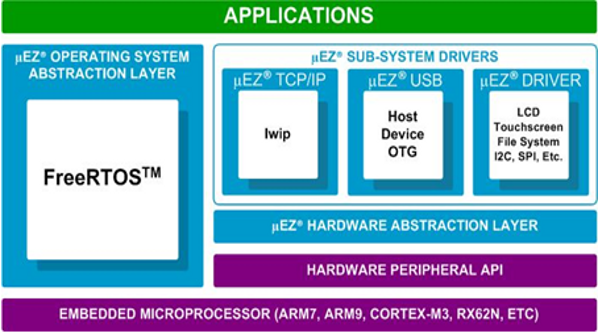
\includegraphics[width=3.2in,height=2.2in,clip,keepaspectratio]{uEZ.png}

Si vuole far notare che uEZ possiede un sistema operativo da poter sfruttare chiamato FreeRTOS, un sistema operativo realtime embedded che offre tutti i servizi utili per gestire concorrenza e sincronizzazione.

Per queste librerie è necessario implementare il porting dell'architettura desiderata, per poi avere un codice "portabile" per tutti i sistemi che utilizzano le stesse librerie per funzionare. Inoltre sono altamente ottimizzate per non sprecare risorse sia di memoria sia energetiche, in modo da progettare un sistema commercializzabile.



\section{Il framework per il caso di studio}
Poiché si vuole dare una metodologia di sviluppo efficiente per la creazione di sistemi con interfaccia utente, è necessario l'utilizzo di un framework. Questo è stato creato unendo le librerie sopra citate per poi creare una struttura software modulare in modo da poter sostituire, eliminare o aggiungere ulteriori moduli software. 

Questo framework permette di scegliere il tipo di interfaccia da utilizzare (per dispositivo cieco o visuale) e, se il sistema scelto lo permette, di avere entrambe le tipologie di interfacce. Fornendo inoltre una procedura standard per poter progettare l'intero sistema, è possibile automatizzare tutta la progettazione con tool automatici. L'unico procedimento non automatico consiste nell'eseguire l'interfacciamento con l'hardware per permettere alle funzioni di livello superiore di interagire con esso.

Il framework si può rappresentare con questo schema:

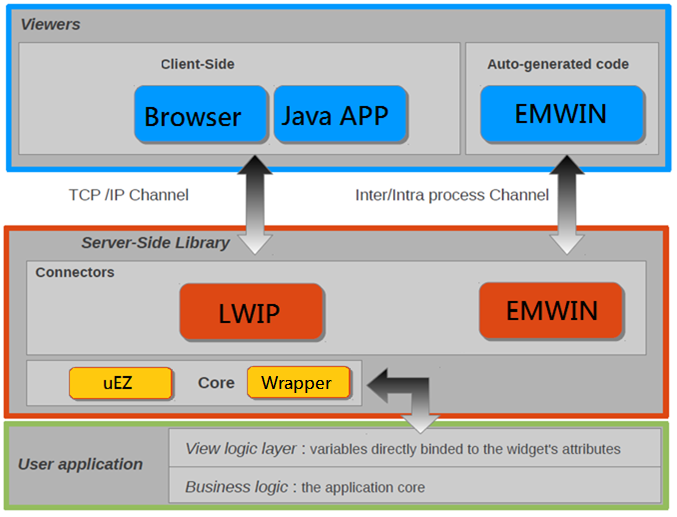
\includegraphics[width=5in,height=2.5in,clip,keepaspectratio]{framework.png}

Si può notare che il core del framework, ovvero ciò che lo fa effettivamente funzionare, è composto da uEZ più un Wrapper che deve gestire le richieste della Business Logic e dello strato che gestisce il comportamento dell'interfaccia; in questo modo, l'intero core sarà portabile e il Wrapper eviterà problemi di \textit{race conditions} per l'accesso alle risorse. 
Al core si collegano due tipi di connettori, uno di rete, ovvero LWIP, e uno di interfaccia grafica locale, ovvero EMWIN. I due connettori hanno il compito di mettere in comunicazione la parte di logica di controllo con la parte Client in cui avverrà la visualizzazione dell'interfaccia, chiamata nello schema "Viewers". La parte di EMWIN si interfaccia tramite le procedure interne della libreria stessa, mentre la parte di LWIP si connette tramite TCP/IP con uno strato applicativo che funge da interprete di comandi e da compositore di risposte.

Si può subito notare che si comporta come un'architettura Client/Server: i Viewers (Client), tramite l'interazione con l'utente, creano dei messaggi da inviare alla logica di controllo, mentre questa tramite i connettori (Server) riceve i messaggi, li elabora e invia la risposta. Quindi il Server è il riquadro con bordo rosso, mentre il Client è il riquadro con bordo azzurro.

Bisogna considerare che può esserci anche la situazione in cui è il Server a dover inviare qualche informazione al Client, poiché si ha sempre una situazione di multitasking in cui si devono controllare oggetti che possono variare autonomamente il loro valore (ad esempio un sensore di temperatura). Quindi, è necessario utilizzare un'architettura Client/Sever con la possibilità da parte del Server di inviare notifiche Push per notificare i Client pur non avendo loro fatto alcuna richiesta. Ciò è anche giustificato dal fatto che bisogna anche rispettare il vincolo di consumo, quindi situazioni di polling non sono ammesse perché presentano un notevole overhead di informazioni inutili, oltre al fatto che la parte di comunicazione di un dispositivo Embedded è quella che consuma più energia.

\subsection{Funzionamento di LWIP}

LWIP offre una versione ridotta del protocollo TCP/IP, quindi manca lo strato HTTP. Su dispositivi di fascia bassa, diventerebbe particolarmente oneroso gestire anche il livello HTTP, sopratutto per il fatto che bisognerebbe implementare e gestire anche l'invio di file che rappresentano pagine Web. Quindi bisogna comunicare con il dispositivo tramite Socket semplici, in modo da garantire richieste asincrone in entrata ed uscita indipendenti.

Nel framework creato, si hanno due situazioni differenti: una richiesta da parte del Client e una notifica da parte del Server.

Nella prima situazione, il Client invia una stringa che corrisponde ad un commando specifico; il comando viene definito dal progettista ed è dipendente dall'applicativo. Questo comando è formato dal tipo di comando, rappresentato da un numero, e dai suoi argomenti (ad esempio: "1 1" può significare "imposta il Led 1 ad ON").

Nella seconda situazione, in accordo con lo standard moderno dei Client per trattare messaggi asincroni, il Server invia un messaggio JSON, che descrive il tipo di messaggio e, in base ad esso, si devono ottenere i contenuti descritti in variabili.

\subsection{Funzionamento di EMWIN}

EMWIN offre una parte di core grafico trasparente e nascosta al progettista, quindi per creare l'interfaccia grafica bisogna semplicemente definire la posizione dei widget ed associarvi un comportamento in base all'interazione che l'utente ha con esso (pressione, rilascio, ecc...).

L'architettura Client/Server con notifiche Push anche in questo caso è rispettata, in quanto la GUI (Client) esegue delle richieste alla Business Logic (Server) tramite le funzioni di libreria, mentre se la Business Logic deve notificare all'interfaccia una modifica, può farlo invocando delle funzioni di libreria della stessa (Push).

\subsection{Funzionamento del Wrapper}

Un ruolo fondamentale per evitare tutti i tipi di conflitti lo ricopre il Wrapper, in quanto ha il compito di processare le richieste e fare in modo che la relativa procedura venga eseguita su tutte le interfacce, senza creare situazioni di conflitti di dati o addirittura di bloccare l'intero sistema.

Il Wrapper appare come un ``multiplexer'' di funzioni: ogni richiesta, prima di essere processata da questo, viene elaborata in modo da renderla comprensibile dal Wrapper; poi, in base all'origine e alla natura della richiesta (se è un comando o una notifica) viene incanalata verso il connettore corrispondente. Oltre ad eseguire i comandi corrispondenti alle richieste, deve gestire i meccanismi di sincronizzazione tra i vari task generati dalle richieste, quindi è in grado di creare semafori, gestirli e distruggerli; in questo modo, la progettazione delle interfacce risulta molto più semplificata ed è compito del Wrapper gestire la sincronizzazione. Si vuol far notare inoltre che la sincronizzazione avviene soprattutto nella fase di inizializzazione delle interfacce, ovvero quando bisogna attendere che i vari Client siano pronti per ricevere i dati con cui popolare l'interfaccia; questo perché l'interfaccia Web sarà sempre più veloce dell'interfaccia su schermo del sistema.

L'architettura con il Wrapper può essere presentata nel dettaglio in questo modo: 

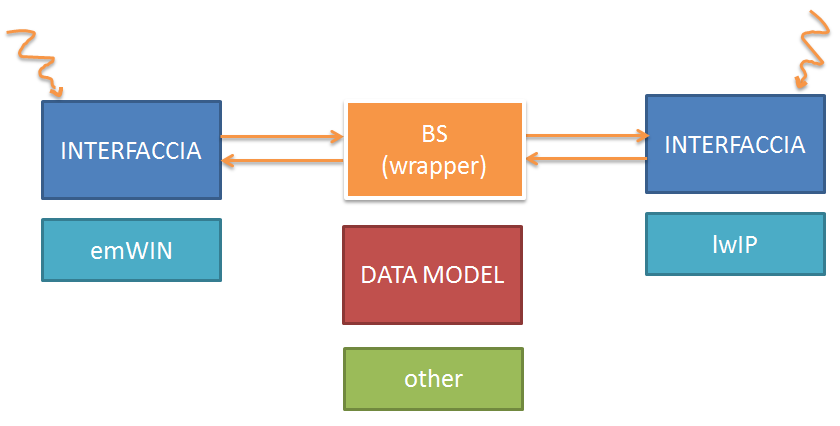
\includegraphics[width=3in,height=2in,clip,keepaspectratio]{Wrapper.png}

Quindi il Wrapper deve aver modo di comunicare con le due diverse interfacce e tenerle sincronizzate, registrando ogni evento generato da queste e notificandolo alla rispettiva opposta.


\section{Metodologia di sviluppo}

\section{Analisi della metodologia}

Si vuole ora analizzare l'utilizzo di questo metodo di progettazione proposto paragonandolo alla progettazione allo stato della pratica. 

Innanzitutto, utilizzando un metodo standard di progettazione come quello proposto (standard nel senso che segue un paradigma di progettazione ben preciso), si è sicuri di proporre un software altamente mantenibile, modulare e soprattutto comprensibile a tutti. Uno dei più grandi problemi delle aziende in cui si progetta software è la comprensione del software generato da progettisti diversi, in quanto ogni progettista che non segue un metodo standard non propone un software facilmente comprensibile ad altri. Oltre a questo, rispettare una metodologia condivisa porta più facilmente all'individuazione di bug e problemi, in quanto bisogna rispettare delle regole di scrittura che sono consolidate nel tempo.

Un fattore che ha portato benefici con questo metodo è la velocità di progettazione, oltre alla semplicità meccanica della scrittura del software: seguire questo metodo utilizzando un framework ha portato ad una progettazione 6 volte più veloce dello stesso software, con debug facile e codice pulito. Avere una struttura molto modulare, piuttosto che codice monolitico tipico dei Sistemi Embedded a fascia bassa, ha portato ad avere questo \textit{speed up} di progettazione.

La creazione di un Wrapper per gestire i problemi di sincronizzazione ha facilitato la gestione sia del modello di sistema sia dell'identificazione di problemi: i problemi più importanti, come la sincronizzazione, risiedono dentro questo modulo e quindi è facile sapere che, qualora ci fosse un deadlock, si trova dentro una chiamata di questo modulo.

Infine, il fatto che la progettazione risulta meccanica, significa che questo framework può essere trasformato in un tool automatico per la generazione e gestione di interfacce grafiche, perché segue una procedura ben precisa per la scrittura di software.

\section{Analisi delle risorse utilizzate}

In accordo con i vincoli precedentemente descritti che un Sistema Embedded di fascia bassa deve rispettare per poterlo rendere un prodotto affidabile, è doveroso considerare quante risorse vengono utilizzare per progettare un sistema di interfaccia utente. Dal momento che questi sistemi permettono esclusivamente di essere programmati con tecnologie altamente ottimizzate, come un binario ottenuto dalla compilazione di codice C, si presume che, in ogni caso, il codice prodotto sia sempre performante; in realtà bisogna considerare che, avendo risorse limitate dal punto di vista di memoria e velocità, bisogna ridurre il più possibile il codice. Sorge quindi il dubbio se effettivamente conviene utilizzare un framework per progettare questi sistemi, in quanto questo può aggiungere codice superfluo per astrarre il più possibile la progettazione, ma, secondo le analisi fatte, in realtà non è così pesante sia dal punto di vista di utilizzo di memoria sia di occupazione di cicli di clock.

Il framework presentato, essendo esclusivamente modulare, non creando quindi ulteriori livelli che eseguono effettive operazioni, occupa solamente più Stack durante l'esecuzione: analizzando staticamente il codice, si può notare che si hanno solamente chiamate a funzione nidificate, in particolare 4 chiamate a funzione per ogni chiamata da parte del Wrapper più 4 chiamate per accedere alle periferiche fisiche da parte del core uEZ, quindi in totale, nel caso pessimo, si occupano 8 livelli di Stack in più rispetto ad un codice senza framework. In questo caso però il compilatore C, con un'opportuna ottimizzazione (per gcc basta il livello 2 di ottimizzazione) da 8 livelli di Stack vengono ridotti a 2, poiché vengono visti come ridondanti e quindi è permessa la riduzione di chiamate. Dal punto di vista invece del tempo di esecuzione, il framework non porta un rallentamento percepibile, in quanto sarebbe dovuto da chiamate a funzione nidificate, però vengono ottimizzate dal compilatore. L'effettivo consumo di risorse, per quanto minimo, è dato dal Wrapper quando deve interpretare e inoltrare le richieste ai diversi Client; questa operazione si presenta come un massiccio ``switch'', quindi ha un'ordine di complessità di \textit{O(n)} nel caso pessimo, quindi potrebbe creare problemi di \textit{realtime} quando si crea un'interfaccia con una grande quantità di widget. Considerando però che gli schermi di questi sistemi spesso non superano i 10 pollici e un'interfaccia utente, secondo gli studi dati dall'interazione uomo-macchina, deve rispettare dei vincoli di dimensione dei widget per permettere un utilizzo facilitato, la variabile \textit{n} nel caso pessimo non raggiungerà mai un valore più alto di 100, quindi è accettabile come computazione.

\subsection{Gestione della sezione critica e Threads}

Per gestire le sezioni critiche, sono stati utilizzati dei semafori binari di uEZ, che si interfacciano con i semafori di FreeRTOS tramite chiamate API. Questi, per risparmiare memoria ed evitare conflitti, vengono creati, inizializzati e distrutti nella main thread del framework, mentre vengono utilizzati dalle thread che devono rispettare la sincronizzazione. Bisogna far notare che i semafori non devono essere utilizzati dalla main thread ma solamente dalle thread concorrenti, in quanto l'intero sistema potrebbe bloccarsi per un tempo indefinito.

Le thread asincrone si devono occupare di molti controlli; alcune sono trasparenti al progettista, ovvero il controllo dello schermo LCD Touch, dell'inizializzazione della parte di rete e della parte di GUI (trasparenti nel senso che il progettista non deve occuparsi di farle partire o di crearle, ma sono già presenti nel core del framework), invece le più importanti, ovvero il controllo dell'interfaccia GUI e il controllo dell'interprete di rete, devono essere definite dal progettista. Queste continuano la loro esecuzione in maniera totalmente asincrona, finchè non devono interagire tra loro tramite il Wrapper; in quel caso, sono state gestite in modo che aspettino che entrambe abbiano completato l'update dell'interfaccia, in modo che la main thread possa proseguire l'esecuzione avendo la consapevolezza che le interfacce siano sincronizzate (quindi che i widget rappresentino lo stesso valore).

\subsection{Gestione della rete}

Poichè la parte di rete consuma molta più energia tra i componenti di un Sistema Embedded, è stato necessario gestirla in modo che non crei problemi di consumi. La scelta di utilizzare LWIP è stata importante in quanto non porta problemi eccessivi di consumo, infatti nulla è stato gestito in polling; il problema potrebbe derivare dalla parte applicativa della rete, ovvero l'interprete di comandi e il generatore di risposte.

L'interprete è stato gestito come un terminale asincrono: si apre una Socket TCP, si esegue una thread che rimane in ascolto non attivamente sulla Socket e, al momento della ricezione del primo carattere che rappresenta il comando, si risveglia la thread e comincia a leggere tutti i caratteri fino al raggiungimento di \textit{new line}. Per fare in modo che la thread si possa risvegliare solo nel momento in cui deve effettivamente funzionare, è stato associato l'interrupt corrispondente al canale RX della porta Ethernet alla thread, che viene prontamente risvegliata al momento della lettura; una volta letto il carattere, assume lo stato dormiente e non consuma energia. In questo modo si ha un grande risparmio energetico, oltre al fatto che si lascia libera la CPU evitando di fare polling sulla porta di lettura. Questo procedimento è reso possibile dalla \textit{netif} proposta da LWIP, che permette, oltre a definire le porte da settare per far funzionare l'hardware della parte di rete, di impostare gli interrupt associati ad essa. 

\section{Conclusione}

Questo documento ha lo scopo di proporre un nuovo metodo di progettazione di sistemi di fascia bassa per l'interazione grafica, proponendo un approccio modulare e automatizzabile tramite un framework. Dalle analisi proposte risulta molto più produttivo utilizzare questo tipo di approccio, piuttosto di non seguire un modello di progettazione di questi sistemi. Sarà interesse futuro continuare questo framework in modo da renderlo commerciale e proporre tools per automatizzare la progettazione tramite esso. 

\ifCLASSOPTIONcaptionsoff
  \newpage
\fi


\end{document}


